\chapter{Сведения из теории нейронных сетей}

\section{Функции потерь и метрики}
\subsection{$F_1$-score}
Метрика $F_1$-score (она же $F_1$-мера) является одной из наиболее предпочтительных метрик для оценки
производительности моделей в задачах с сильным дисбалансом классов.

$F_1$-мера учитывает как точность, так и полноту. Это гармоническое среднее между
точностью (precision) и полнотой (recall) (см. формулу \ref{eq:f1score}), что позволяет
учитывать как количество правильно классифицированных положительных случаев,
так и способность модели обнаруживать все положительные случаи. Так же $F_1$-мера
остается стабильной при изменении соотношения классов в выборке данных, что
делает ее надежной метрикой для задач с сильным дисбалансом классов.

\begin{align}
	precision & = \frac{TP}{TP + FP}, \: recall = \frac{TP}{TP + FN}, \: \text{где} \\
	          & \begin{cases}
		            TP = \: \text{true positive}  \\
		            FP = \: \text{false positive} \\
		            FN = \: \text{false negative}
	            \end{cases}, \: \text{а} \\
	F_1score  & = 2 \cdot \frac{precision \cdot recall}{precision + recall} = \frac{TP}{TP + 0.5(FP + FN)}
	\label{eq:f1score}
\end{align}

\subsection{Функции потерь}
\subsubsection{Бинарная кроссэнтропия}

Бинарная кросс-энтропия является широко применяемой функцией потерь для задач
классификации и обладает следующими преимуществами:

\begin{enumerate}
	\item Чувствительность к вероятностям: Бинарная кросс-энтропия учитывает
	вероятности предсказанных классов, а не только факт совпадения меток. Это
	позволяет модели учитывать уверенность в своих предсказаниях и лучше
	интерпретировать результаты.

	\item Легко интерпретируема: Значения функции потерь бинарной
	кросс-энтропии имеют простой смысл: они означают степень несоответствия
	между истинными метками и предсказанными вероятностями, что делает
	интерпретацию процесса обучения и оценку модели более прозрачными.

	\item Подходит для задач сбалансированных и несбалансированных классов:
	Бинарная кросс-энтропия хорошо работает как для задач с равным количеством
	примеров каждого класса, так и для задач с несбалансированными классами.

	\item Применима в градиентных методах оптимизации: Бинарная кросс-энтропия
	гладкая и дифференцируемая функция, что позволяет использовать градиентные
	методы оптимизации для её минимизации. Так же важным ее свойством является
	то, что она выпуклая, что значительно упрощает оптимизацию градиентными
	методами.


\end{enumerate}

Формула выглядит следующим образом:

\begin{equation}
	BCE = - \frac{1}{N} \sum_{i=1}^{N} \left[ y_i \cdot \log(\hat{y}_i) + (1 - y_i)
		\cdot \log(1 - \hat{y}_i) \right]
	\label{eq:bce}
\end{equation}

\noindent $N$ --- размер входного вектора, $\hat{y}_i$ --- $i$-ая компонента
предсказания, $y_i$ --- $i$-ая компонента истины.

\subsubsection{DICE}

Функция потерь Dice хорошо себя зарекомендовала в задачах сегментации благодаря
следующим свойствам:

\begin{enumerate}

	\item Точное выделение границ объектов: Функция потерь Dice позволяет
	модели точно выделять границы объектов даже на участках сложных форм. Это
	обеспечивает более чёткую сегментацию.

	\item Устойчивость к несбалансированным классам: Dice loss хорошо
	справляется с задачами, где классы несбалансированы.

	\item Математическая простота и эффективность: Dice loss имеет простую
	математическую формулу и легко оптимизируется в процессе обучения модели.

\end{enumerate}

Формула выглядит следующим образом:

\begin{equation}
	DICE = 1 - 2 \cdot \frac{\sum_{i=1}^{N} y_i \cdot \hat{y}_i}{\sum_{i=1}^{N} \left[y_i + \hat{y}_i \right] + \epsilon}
\end{equation}


\noindent $N$ --- размер входного вектора, $\hat{y}_i$ --- $i$-ая компонента
предсказания, $y_i$ --- $i$-ая компонента истины, $\epsilon$ --- небольшое
число для избежания деления на 0.

\section{Инструменты для улучшения качества предсказания и ускорения обучения}

\subsection{Пакетная нормализация}

Пакетная нормализация (batch normalization) - это метод нормализации данных
внутри нейронной сети, который помогает ускорить обучение и повысить его
стабильность. Суть пакетной нормализации заключается в том, что для каждого
пакета данных вычисляются среднее значение и стандартное отклонение по всем
нейронам в слое. Затем входные данные нормализуются путем вычитания среднего
значения и деления на стандартное отклонение. Пакетная нормализация также
вводит два новых параметра для каждого слоя: параметр сдвига (shift) и параметр
масштабирования (scale). Эти параметры позволяют нейронной сети сохранять
возможность представления различных распределений данных и настраивать их по
мере обучения.

Сам алгоритм пакетной нормализации:
\begin{align*}
	z^{(i)} & = \gamma \otimes \hat x^{(i)} + \beta, \text{где}        \\
	\hat x^{(i)} = \frac{x^{(i)} - \mu_B}{\sqrt{\sigma^2_B + \xi}}, \qquad
	\mu_B   & = \frac{1}{m_B} \sum\limits_{i = 1}^{m_B}x^{(i)}, \qquad
	\sigma_B^2 = \frac{1}{m_B} \sum\limits_{i = 1}^{m_B}(x^{(i)} - \mu_B)^2
\end{align*}

\begin{align*}
	z^{(i)}      & \: \text{ --- результат операции: это отмасштабированная и сдвинутая версия входов}  \\
	\gamma       & \: \text{ --- выходной параметр --- масштаб для слоя}                                \\
	\otimes      & \: \text{ --- поэлементное умножение векторов}                                       \\
	\hat x^{(i)} & \: \text{ --- вектор отцентрированных и нормализованных входов для экземпляра} \: i  \\
	\beta        & \: \text{ --- выходной параметр --- сдвиг для слоя}                                  \\
	\mu_B        & \: \text{ --- вектор средних входа, посчитанных по всему пакету}                     \\
	\sigma_B     & \: \text{ --- вектор стандартных отклонений входа, так же считается по всему пакету} \\
	x            & \: \text{ --- вход}                                                                  \\
	m_B          & \: \text{ --- количество элементов в пакете}                                         \\
	\xi          & \: \text{ --- небольшое число для того, чтобы избежать деления на 0}
\end{align*}

\subsection{Исключение}

Dropout, или метод исключения, доказал свою эффективность как мощное средство
регуляризации нейронных сетей \cite{dropout-is-good}. Основная идея метода
заключается в том, что на этапе обучения случайным образом отключаются
некоторые нейроны с указанной вероятностью в каждом пакете данных (см. рис.
\ref{fig:dropout}). По сути это позволяет обучать не одну модель, а ансамбль,
где каждый компонент обучается на своём поднаборе данных. Таким образом,
достигается некая аппроксимация алгоритма бэггинга, который, однако, выходит за
рамки данного обсуждения (дополнительную информацию можно найти в
\cite{goodfellow}).

\begin{figure}[!htb]
	\centering
	\caption{Пример исключения на слое max pool}
	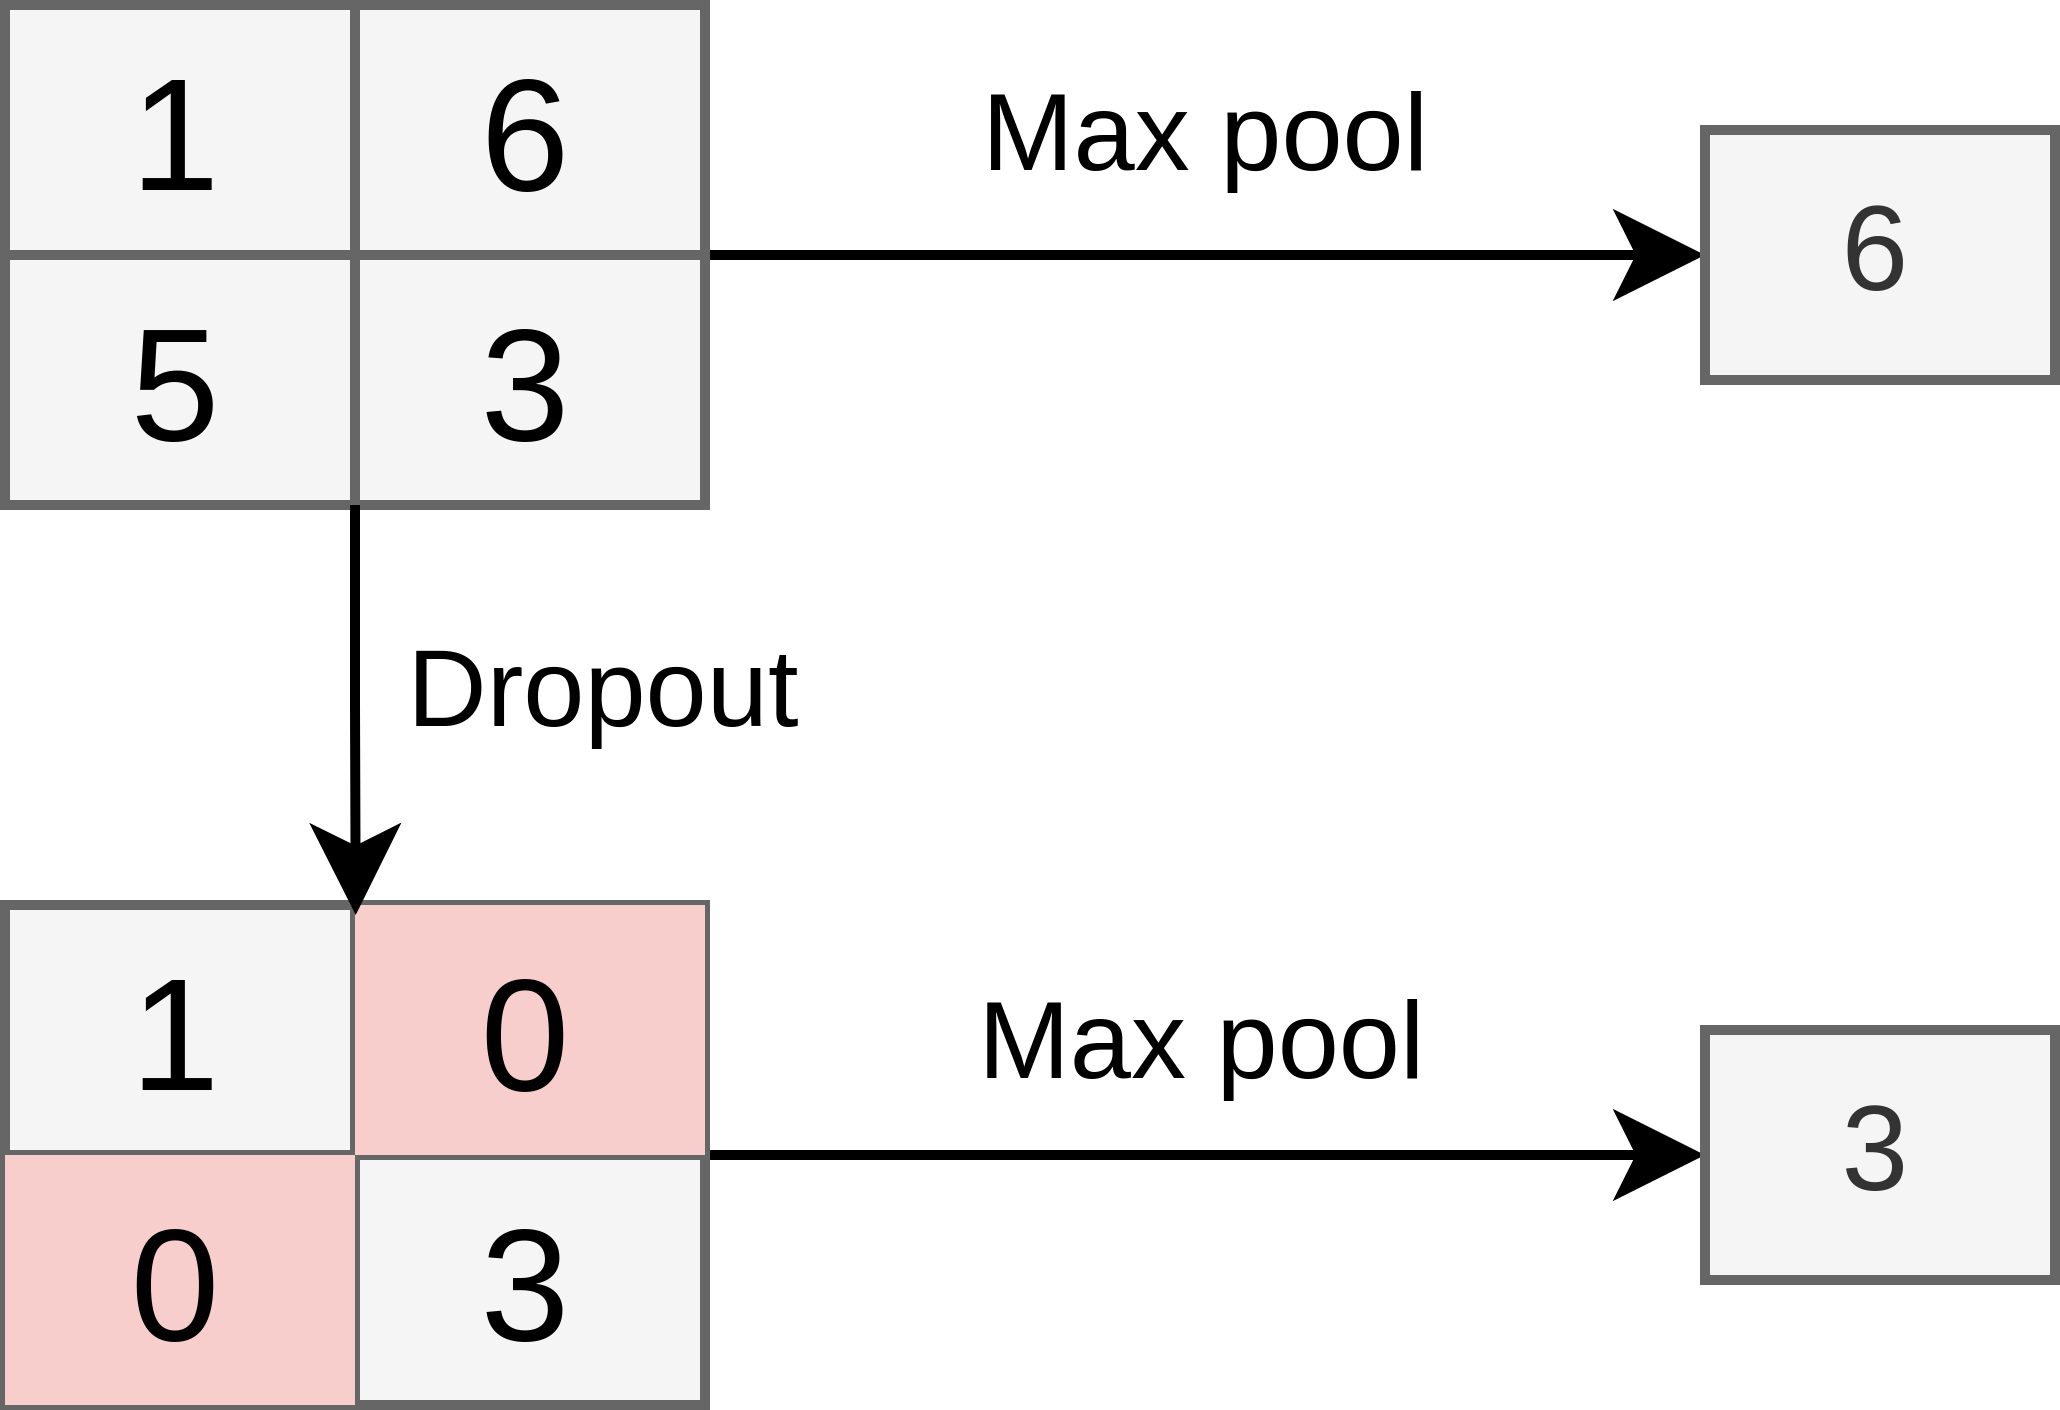
\includegraphics[width=0.4\textwidth]{dropout.png}
	\label{fig:dropout}
\end{figure}

\subsection{Сверточные слои}

Слой свертки, согласно \cite{goodfellow}, придает стабильность предсказывающему
алгоритму, делая его устойчивым к местным изменениям, таким как сдвиги,
повороты и растяжения, а также существенно сокращает размеры входных данных,
поступающих в нейронную сеть. Проще говоря, этот слой выделяет паттерны на
данных, поступающих на его вход. Он располагается в самом начале нейронной сети
и действует как кодировщик, предоставляя нейросети некоторое осмысленное
представление входных данных.

\subsection{Остаточные связи}
Остаточные связи \cite{residual} --- это дополнительные связи между блоками
в нейронной сети (см. рис. \ref{fig:residual}). Данные связи помогают бороться с проблемой
затухающих градиентов, которая возникает в глубоких нейронных сетях из-за
специфики работы алгоритма обратного распространения ошибки, используемого для
обучения нейросети.

\begin{figure}[!htb]
	\centering
	\caption{Пример остаточной связи. F --- функция активации, x --- вход.}
	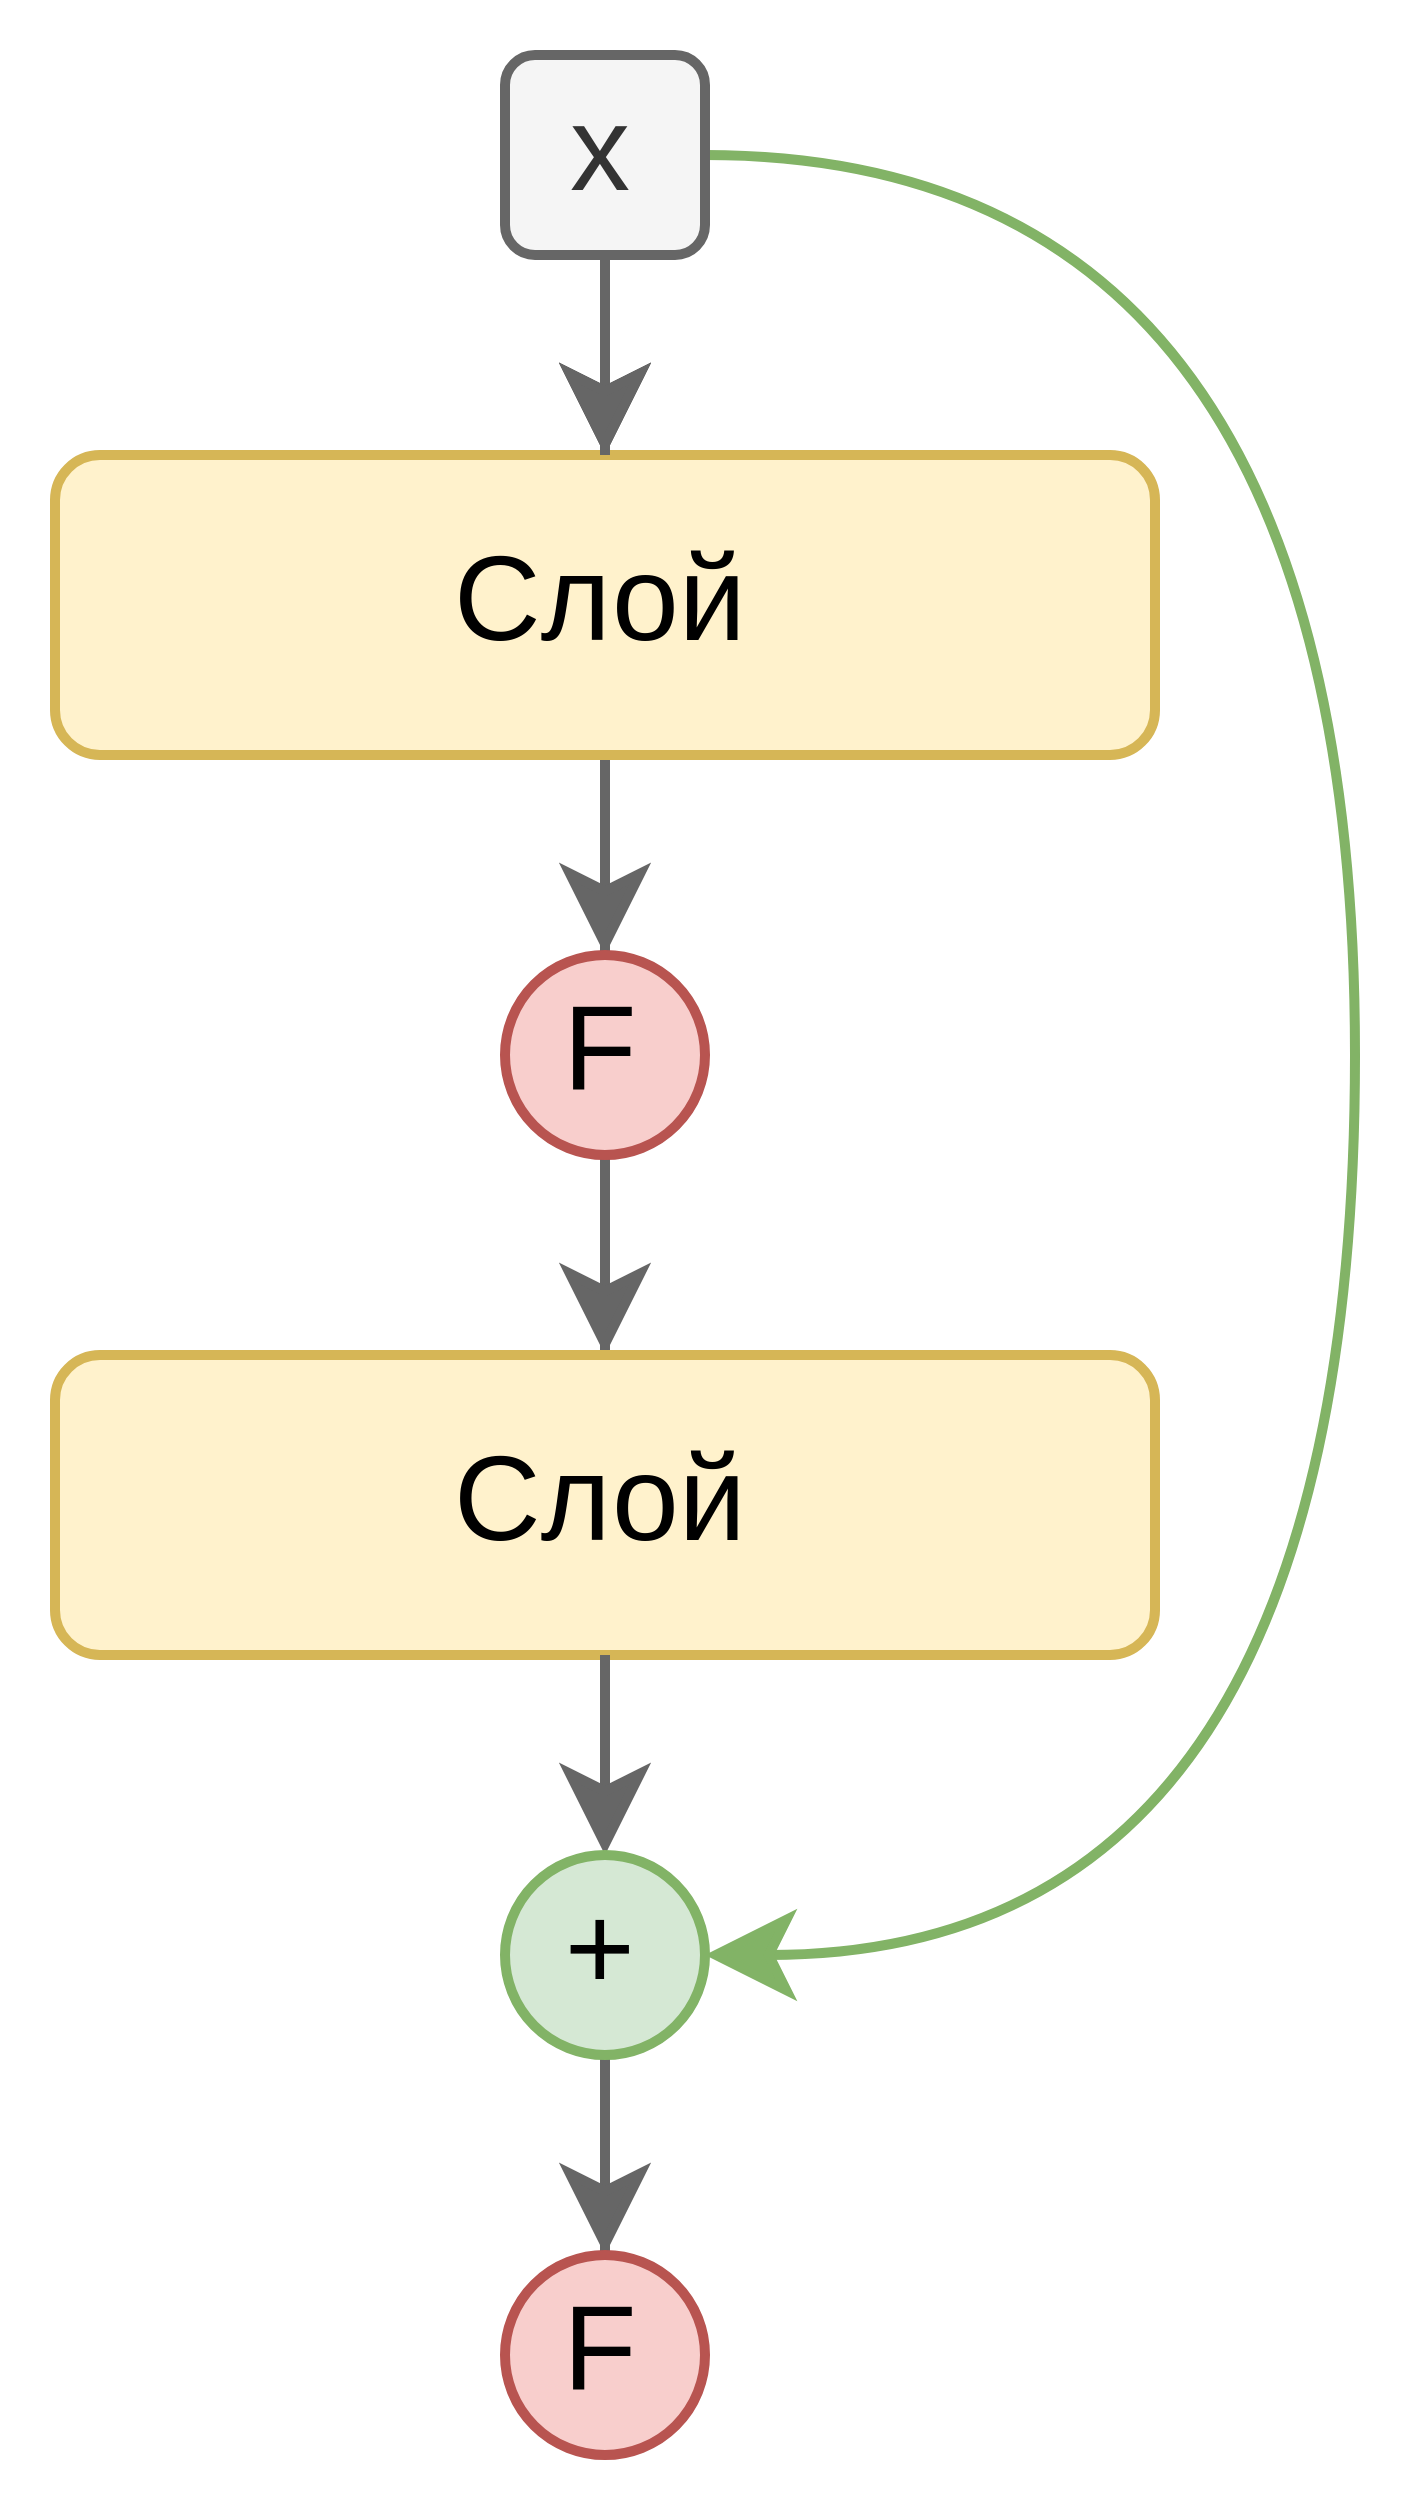
\includegraphics[width=0.25\textwidth]{residual}
	\label{fig:residual}
\end{figure}
